\documentclass[hyperref]{ctexart}
\usepackage[left=2.50cm, right=2.50cm, top=2.50cm, bottom=2.50cm]{geometry} %页边距
\usepackage{helvet}
\usepackage{amsmath, amsfonts, amssymb} % 数学公式、符号
\usepackage[english]{babel}
\usepackage{graphicx}   % 图片
\usepackage{url}        % 超链接
\usepackage{bm}         % 加粗方程字体
\usepackage{multirow}
\usepackage{booktabs}
\usepackage{algorithm}
\usepackage{algorithmic}
\renewcommand{\algorithmicrequire}{ \textbf{Input:}}       
\renewcommand{\algorithmicensure}{ \textbf{Initialize:}} 
\renewcommand{\algorithmicreturn}{ \textbf{Output:}}     
%算法格式
\graphicspath{{figure/}}
\usepackage{fancyhdr} %设置页眉、页脚
\pagestyle{fancy}
\lhead{}
\chead{}
\rhead{红外荧光光谱}
\lfoot{}
\cfoot{\thepage}
\rfoot{}
\usepackage{hyperref} %bookmarks
\hypersetup{colorlinks, bookmarks, unicode} %unicode
\usepackage{multicol}
\title{\textbf{红外荧光光谱实验}}
\author{\sffamily PB19000132 苗立扬}
\date{}
\begin{document}
	\maketitle
	\noindent{\bf 摘要:}
	光照射到某些原子时,光的能量使原子核周围的一些电子从基态跃迁到激发态。激发态不稳定,所以会恢复基态,当电子由激发态恢复到基态时,能量会以光的形式释放,称为荧光。荧光因为能够揭露物质原子内部电子能层的信息,故常用于物质的鉴别,在生产生活中用途广泛。本次实验中,我们测量两种最常见的物质:稀土元素材料与有机材料的荧光光谱。我们分析他们的荧光光谱的不同特征,并为这两种材料的鉴别提出一种可行方案。\\
	\noindent{\bf 关键词: }荧光光谱、物质鉴别、光谱分析
	\begin{multicols}{2}
		\section{引言}
		1852年Stokes在考察奎宁和叶绿素的荧光时,用分光计观察到荧光波长比入射光波长稍长些。经过判明,这种现象不是由光的漫射作用引起的,而是这些物质在吸收光能后重新放射出的不同波长的光。因此,他引入荧光是光发射的概念。
		
		物体经过较短波长的光照,把能量储存起来,然后缓慢放出较长波长的光,放出的这种光就叫荧光。如果把荧光的能量--波长关系图作出来,那么这个关系图就是荧光光谱。荧光光谱当然要靠光谱检测才能获得。
		
		高强度激光能够使吸收物质中相当数量的分子提升到激发量子态。因此极大地提高了荧光光谱的灵敏度。以激光为光源的荧光光谱适用于超低浓度样品的检测,例如用氮分子激光泵浦的可调染料激光器对荧光素钠的单脉冲检测限已达到10-10摩尔/升,比用普通光源得到的最高灵敏度提高了一个数量级。
		
		荧光光谱有很多,如原子光谱1905年,Wood首先报道了用含有NaCl的火焰来激发盛有钠蒸气的玻璃管,并得到了D线的荧光,被Wood称为共振荧光。在Mitchell及 Zemansky和Pringsheim的著作里讨论了某些挥发性元素的原子荧光。火焰中的原子荧光则是Nichols和Howes于1923年最先报道的,他们在Bunsen焰中做了Ca、Sr、Ba、Li及Na的原子荧光测定。从1956年开始,Alkenmade利用原子荧光量子效率和原子荧光辐射强度的测定方法,以及用于测量不同火焰中钠D双线共阵荧光量子效率的装置,预言原子荧光可用于化学分析。 1964年,美国的Winefordner和Vickers提出并论证了原子荧光火焰光谱法可作为一种新的分析方法,同年,Winefordner等首次成功地用原子荧光光谱测定了Zn、Cd、Hg。有色散原子荧光仪和无色散原子荧光仪的商品化,极大地推动了原子荧光分析的应用和发展,使其进入一个快速发展时期。
		
		荧光光谱包括激发谱和发射谱两种。激发谱是荧光物质在不同波长的激发光作用下测得的某一波长处的荧光强度的变化情况,也就是不同波长的激发光的相对效率;发射谱则是某一固定波长的激发光作用下荧光强度在不同波长处的分布情况,也就是荧光中不同波长的光成分的相对强度。
		
		原子荧光可分为 3类:即共振荧光、非共振荧光和敏化荧光,其中以共振原子荧光最强,在分析中应用最广。共振荧光是所发射的荧光和吸收的辐射波长相同。只有当基态是单一态,不存在中间能级,才能产生共振荧光。非共振荧光是激发态原子发射的荧光波长和吸收的辐射波长不相同。非共振荧光又可分为直跃线荧光、阶跃线荧光和反斯托克斯荧光。直跃线荧光是激发态原子由高能级跃迁到高于基态的亚稳能级所产生的荧光。阶跃线荧光是激发态原子先以非辐射方式去活化损失部分能量,回到较低的激发态,再以辐射方式去活化跃迁到基态所发射的荧光。直跃线和阶跃线荧光的波长都是比吸收辐射的波长要长。反斯托克斯荧光的特点是荧光波长比吸收光辐射的波长要短。敏化原子荧光是激发态原子通过碰撞将激发能转移给另一个原子使其激发,后者再以辐射方式去活化而发射的荧光。
		
		荧光光谱具有如下特点:
		
		灵敏度高:荧光分析的最大特点是灵敏度高,通常情况下要比分光光度计的灵敏度高出2-3个数量级。
		
		选择性强:包括激发光谱和发射光谱,在鉴定物质时,通过选择波长可以使分子荧光分析有多种选择。
		
		试样量少和方法简便。
		
		能提供比较多的物理参数:如激发光谱、发射光谱、荧光强度、量子产率、荧光寿命、荧光偏振等参数。这些参数反映了分子的各种特性,并通过它们可以得到被检测分子的更多信息。
		\section{实验原理}
		\subsection{荧光的产生}
		光照射到某些原子时,光的能量使原子核周围的一些电子从基态跃迁到激发态。激发态不稳定,所以会恢复基态,当电子由激发态恢复到基态时,能量会以光的形式释放,所以产生荧光。
		
		该跃迁分为多种,分别具备如下的特点:
		\begin{itemize}
			\item	基态(S0)→激发态(S1、S2、激发态振动能级)的跃迁:
			\begin{enumerate}
				\item	吸收特定频率的辐射;
				\item	量子化;
				\item	跃迁一次到位;
			\end{enumerate}
			\item	激发态(S1、S2、激发态振动能级)→基态(S0)的跃迁:
			\begin{enumerate}
				\item	多种方式和途径;
				\item	速度最快、激发态寿命最短的途径占优势;
				\item	我们着重考察激发态→基态的能量传递途径。如图所示:
			\end{enumerate}
		\end{itemize}
		
			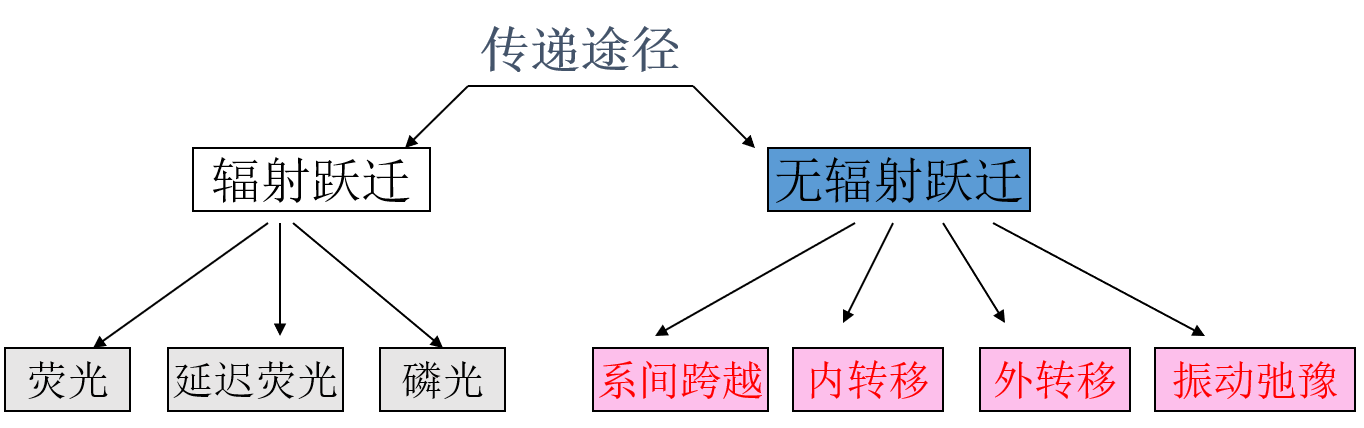
\includegraphics[width = 0.75\linewidth]{propagation_approach.png}
			
	
		由图,激发态停留时间短、返回速度快的途径,发生的几率大,发光强度相对大。
		因此我们着重考虑发光强度最大的荧光。
		
		荧光发射:电子由第一激发单重态的最低振动能级→基态(多为 S1→ S0跃迁),发射波长为$\lambda'_2$的荧光,持续时间在$10^{-7}s\~10^{-9}s$ 。发射荧光的能量比分子吸收的能量小。
		
		\subsection{荧光激发光谱与荧光发射光谱}
		任何因荧光化合物都具有两种特征光谱∶激发光谱和发射光谱。
		\subsubsection{荧光激发光谱}
		荧光激发光谱(激发光谱),就是通过测量荧光体的发光通量随波长变化而获得的光谱,它反映了不同激发光引起荧光的相对效率。激发光谱可供鉴别荧光物质,在进行荧光测定时供选择适宜的激发波长。
		\subsubsection{荧光发射光谱}
		荧光发射光谱又称荧光光谱,如果激发光的波长和强度保持不变,而让荧光物质所产生的荧光通过发射单色器后,照射于检测器上,扫描发射单色器并检测各种波长下相应的荧光强度,然后通过记录仪记录荧光强度对发射波长的的关系曲线,所得到的谱图,称为荧光光谱。
		
		荧光光谱表示在所发射的荧光中各种波长组分的相对强度。荧光光谱可供鉴别荧光物质,并作为在荧光测定时选择适当的测定波长或滤光片的根据。
		
		本次实验,我们着重研究样本的荧光
		
		
		
		
		
		
		
		
		\section{实验仪器与实验步骤}
		\paragraph{实验仪器}
		\subparagraph{荧光光谱仪}
		仪器结构如下图所示:
		
		
		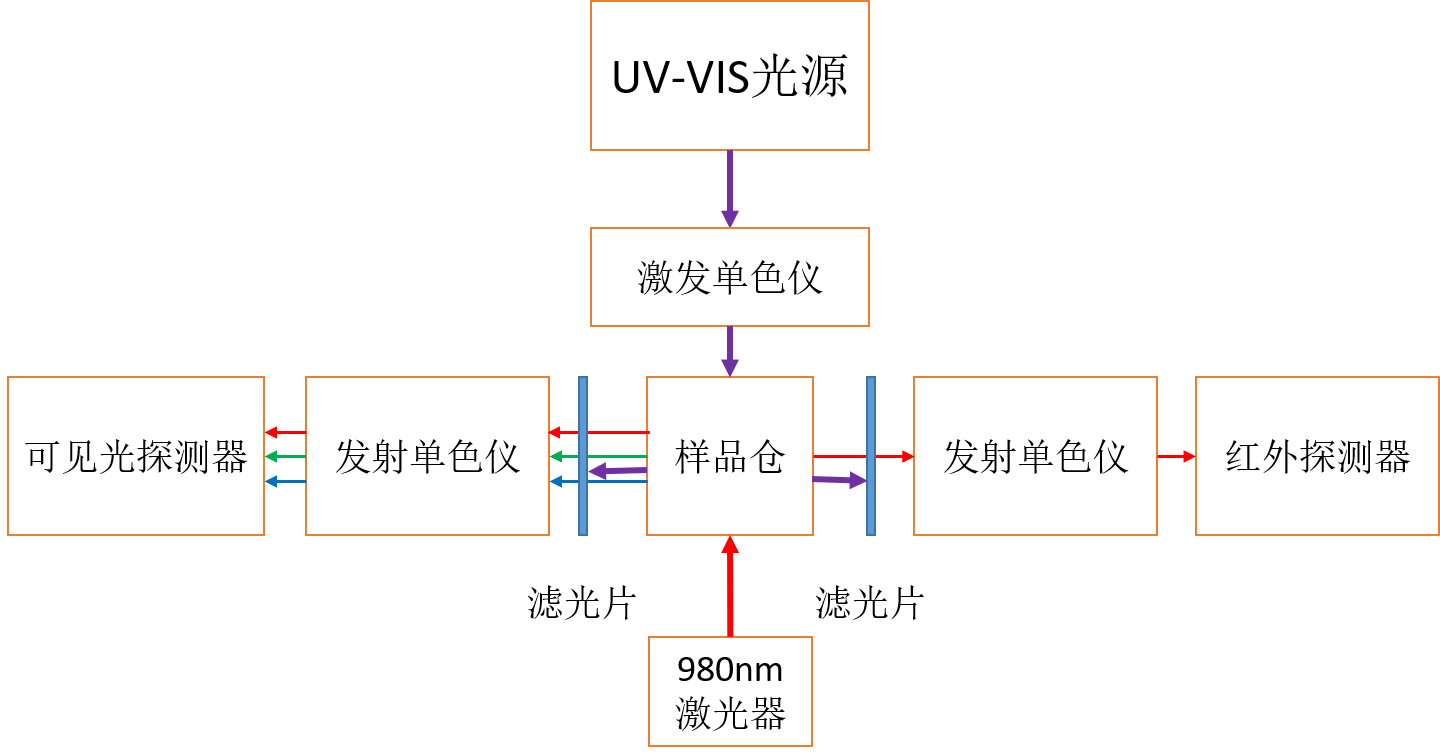
\includegraphics[width = 0.75\linewidth]{apparatus_stru.png}
		
		
		利用UV-VIS光源以及激发单色仪可以得到较好的单色光,范围大致在 间,激光照射位于
		样品仓的样品,样品发出的光通过发射单色仪,并通过探测器,即可得到其发射光谱。

		
		\subparagraph{滤光片}
		滤光片是使待定波长的光通过,其他波段的光反射或衰减的光学元件。其优点为具有高峰值透射率,平
		坦的通带光谱,在很宽的波段范围内具有极好的截止,并且湿温度稳定性较好。滤光片有多种分类。本次实验中,我们选取波长350nm的长波截止滤光片,只有 波长大于350nm的光可以通过。
		
		
		
		\paragraph{实验步骤}
		1、粗测发射谱:根据吸收谱确定激发波长,或直接选用能量较高的蓝紫光(这里选取 )作为
		
		
		2、激发波长,测试预期波长范围的发射光谱。
		测试激发谱:根据发射谱确定发射波长,测试不同波长激发下该发射波长的荧光强度。
		
		
		3、测试发射谱:根据激发谱确定最佳激发波长,测试发射谱。

	
		
		\section{实验图像分析}
		\subsection{稀土材料的发射光谱}
		首先考虑波长为 $350nm$ 的激发光,并且入口狭缝为 $5nm$ ,测量其在可见光范围内的发射光谱。注意到实验中使用了长波截至滤光片,只有波长大于 $350nm$ 的光可以通过,因此发射光谱测量范围设置为为 $400-700nm$ ,步长为 $1nm$ 。由此可以得到如下的发射光谱:
		
		
		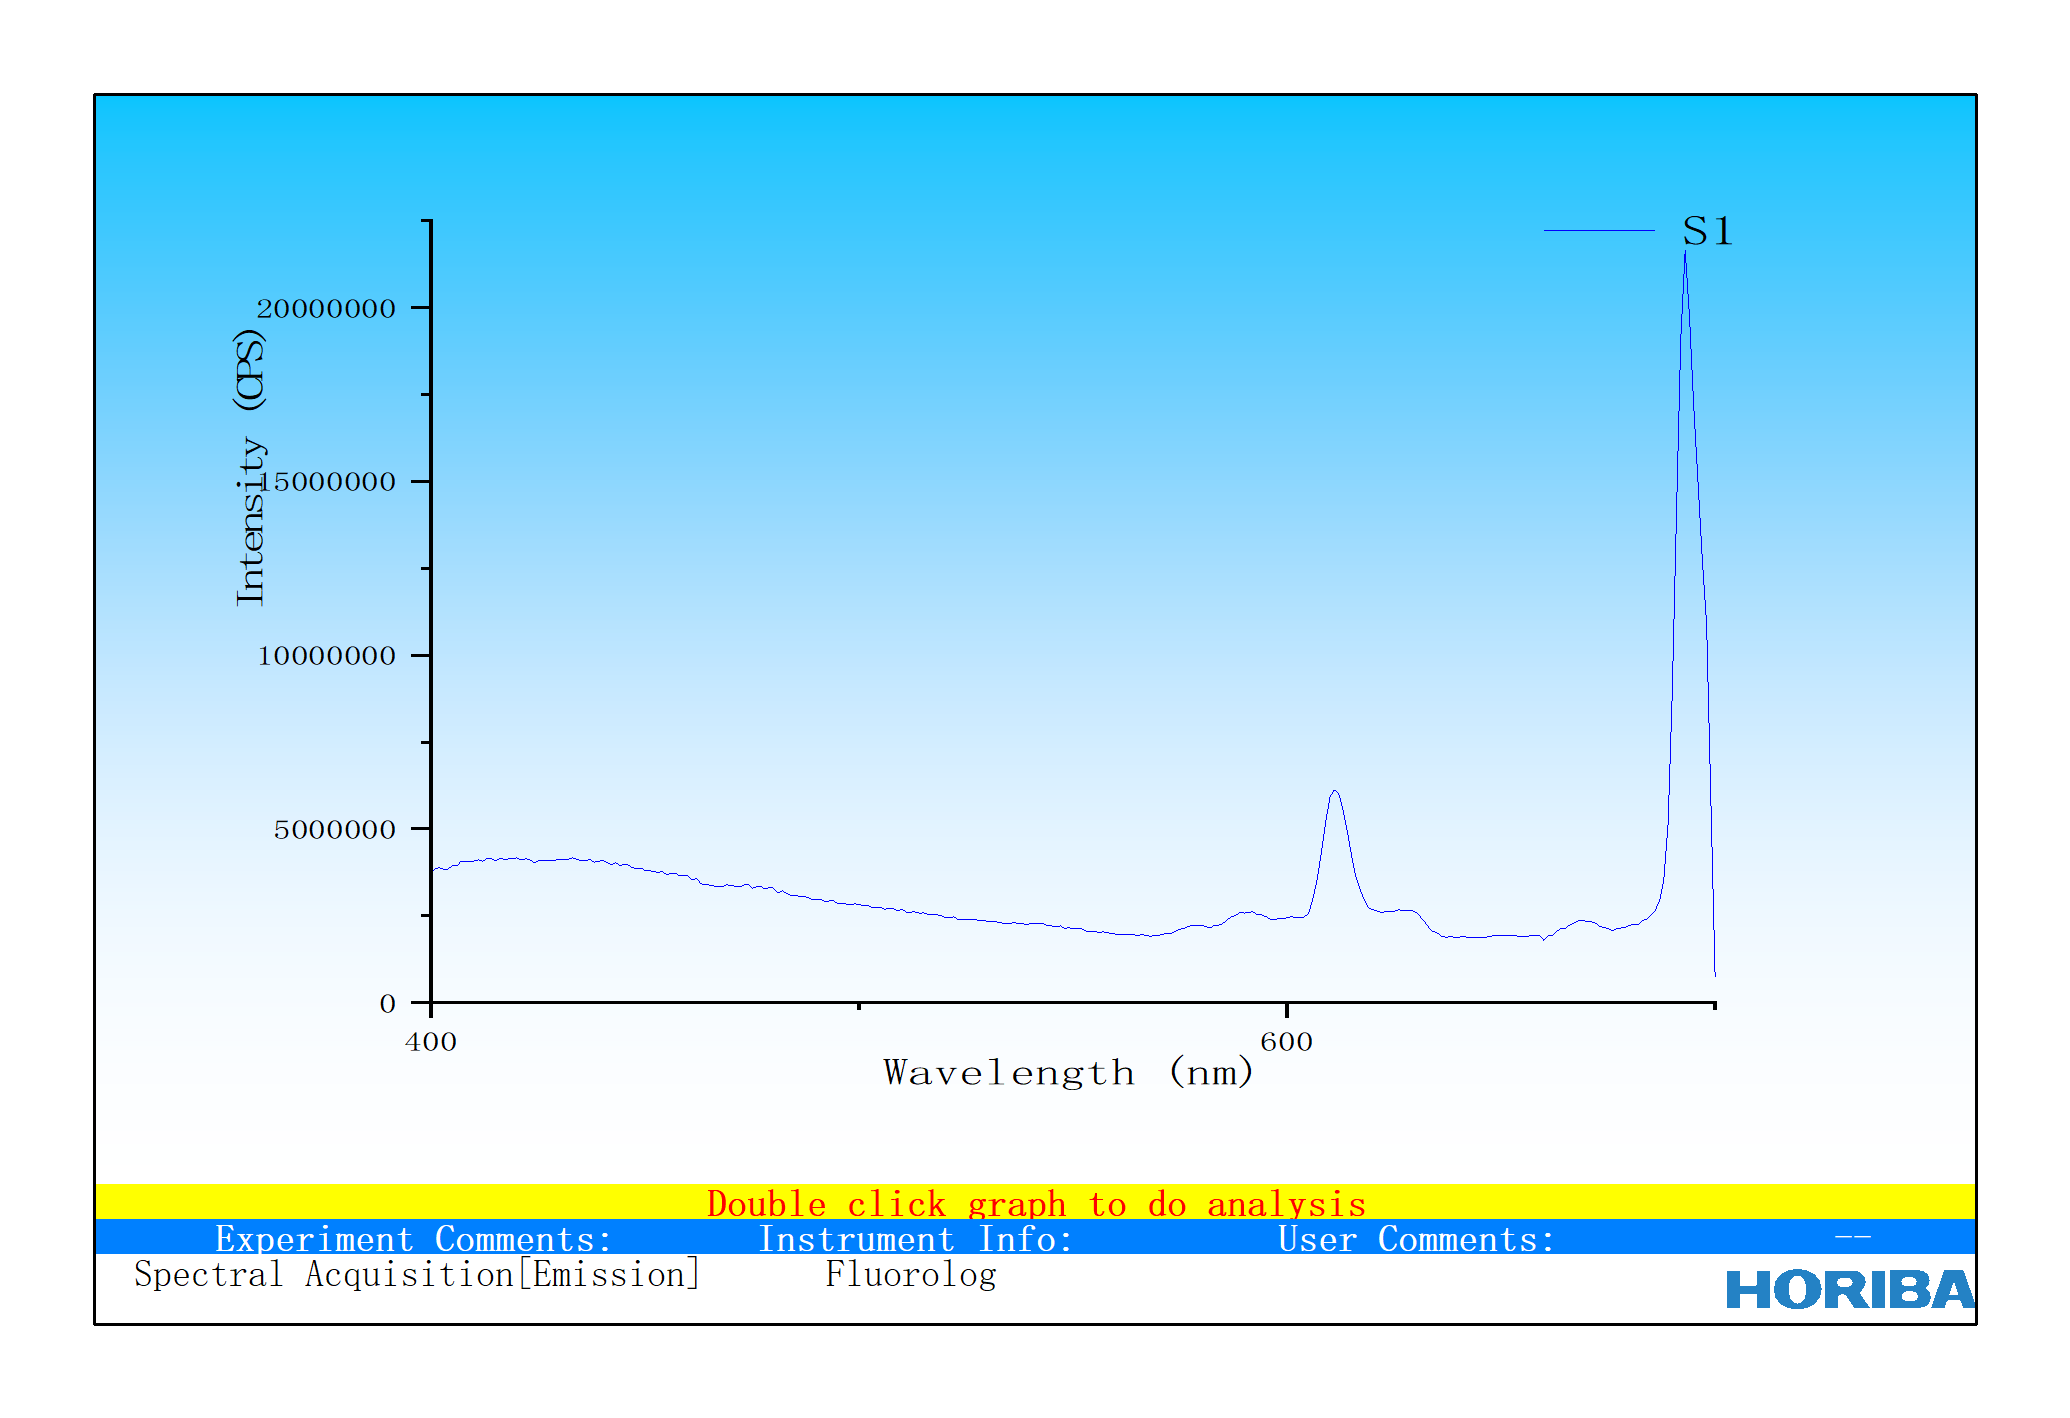
\includegraphics[width = 0.75\linewidth]{RE_Emission_Spectroscopy_400-700_350.png}
		
		可见,光谱有两个峰值,分别位于 $611nm$ 与 $695nm$ 处,不过 $695nm$ 波长处的峰值需要排除,这是因为实验中使用了 $350nm$ 的激发光,这会导致 $700nm$ 左右会有一个较大的峰值,这个峰值来源于激发光被材料反射,而并不来源于样品本身的发射光谱,因此需要将其排除;同时,在波长较短的时候,可以发现其光强较小,所以可以不必关注。为此,实验中修正发射光谱的测量范围为 $ 550-670nm$ ,步长为 $1nm$ ,可以得到如下的发射光谱:
		
		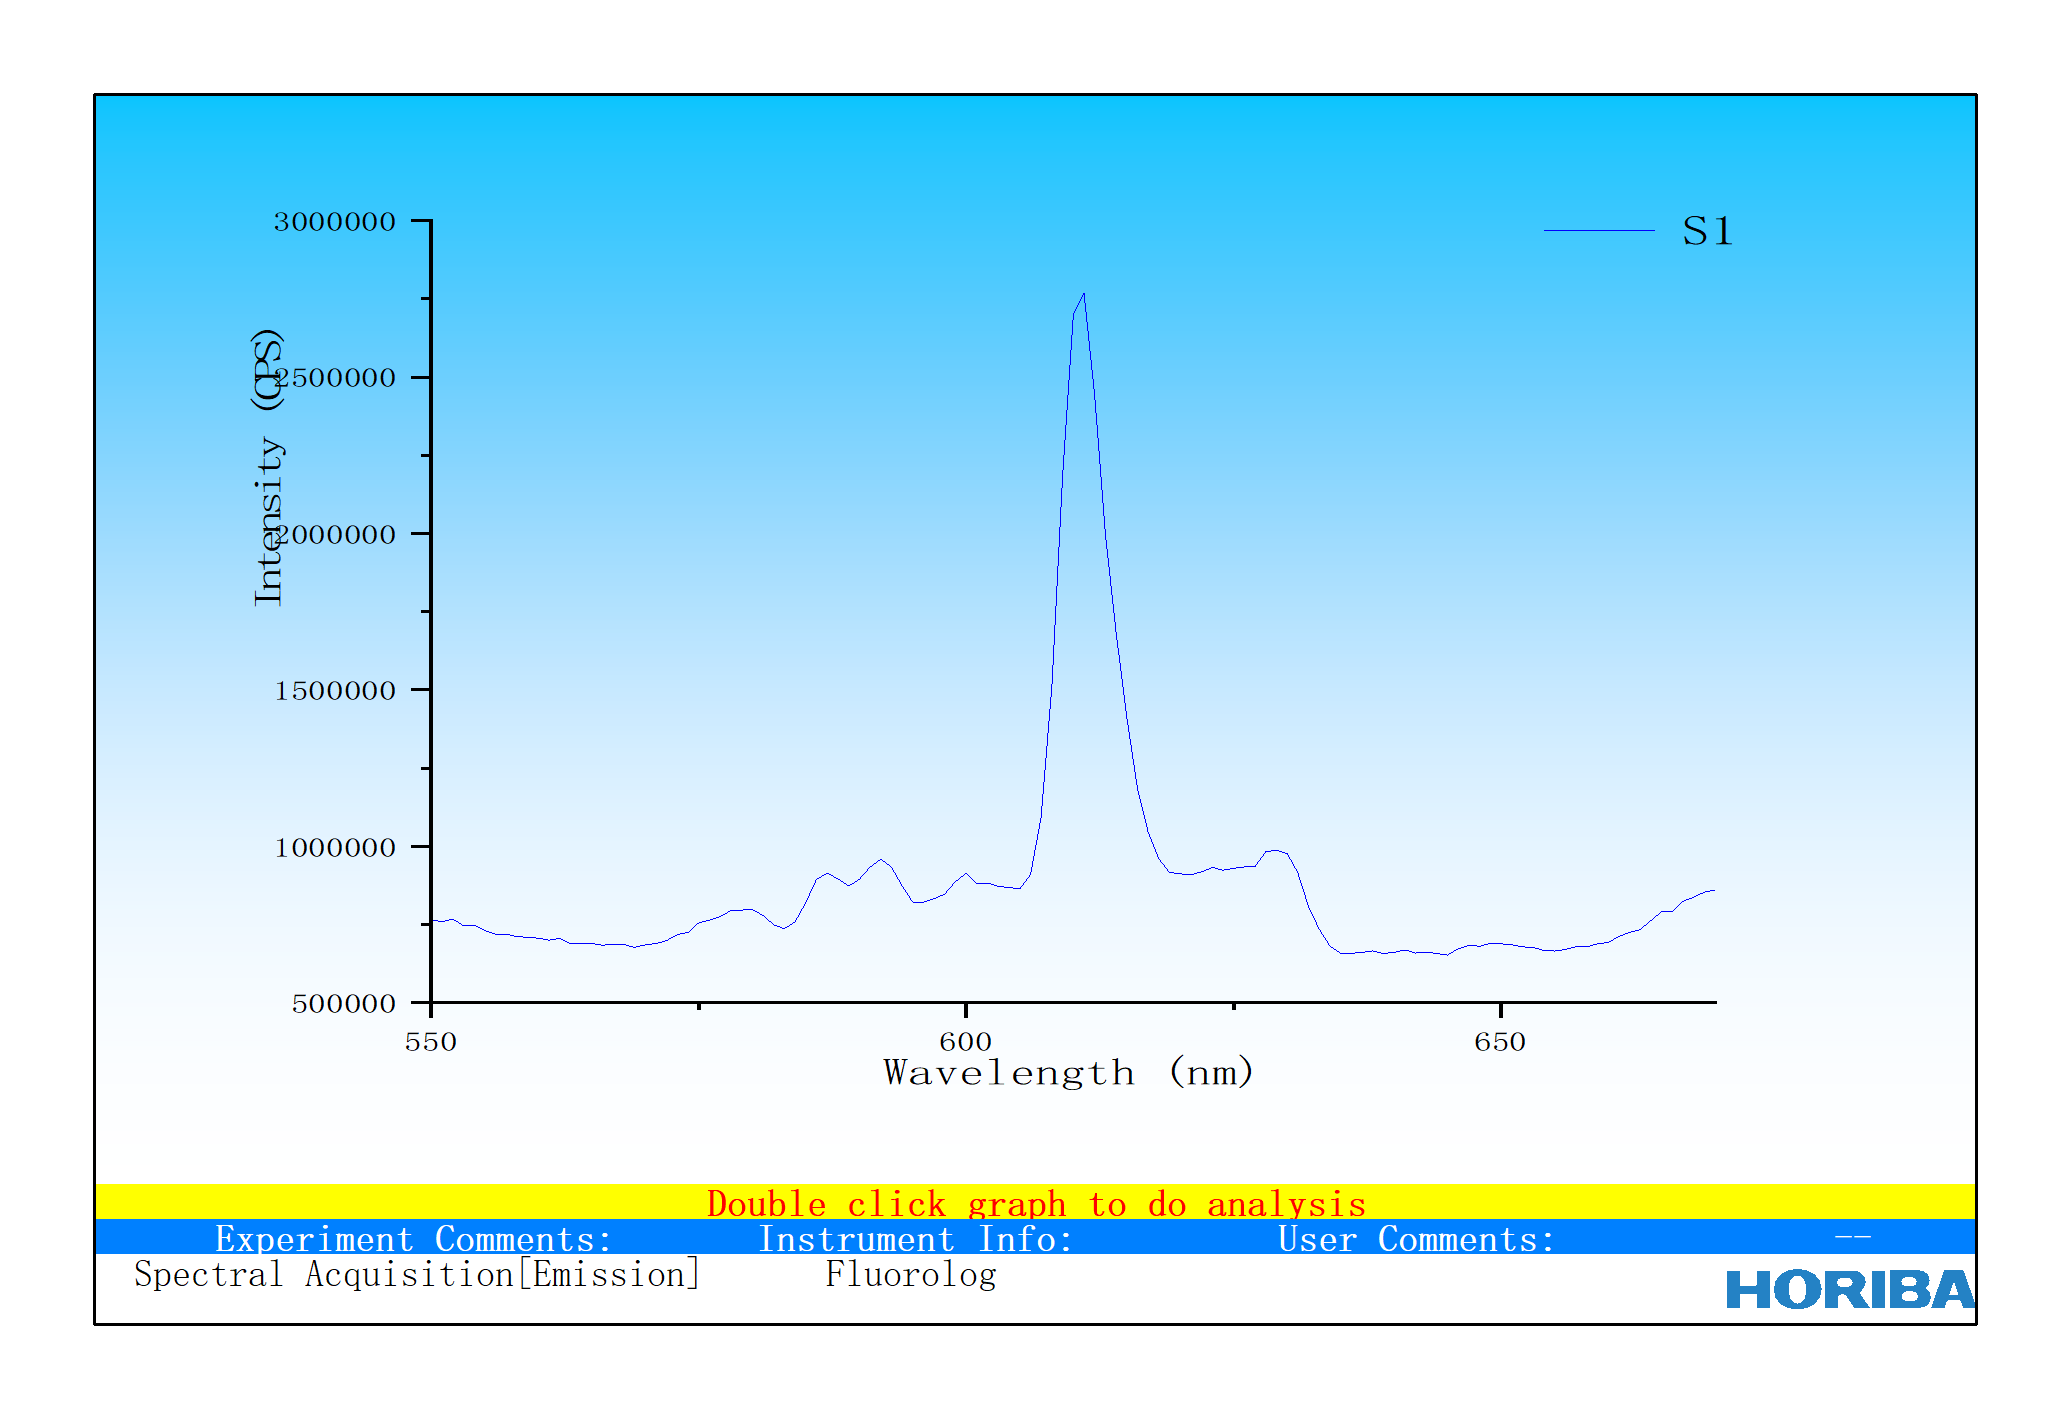
\includegraphics[width = 0.75\linewidth]{RE_Emission_Spectroscopy_550-670_350.png}
		
		这样就可以得到,在 $350nm$ 的激发波长下,稀土样本在可见光范围($550-670nm$)的发射光谱,可以发现在 $611nm$ 附近仍有一些小的峰值,这些峰值是真实的发射光谱的峰值,或是一些噪声,这是无法确定的。因此继续改变激发波长,测量不同激发波长下,发射光谱在$611nm$ 处的峰值的强度。设置激发波长为 $260-600nm$ ,步长为 $1nm$ ,测量 $611nm$ 处的发射光谱的强度,可以得到:
		
		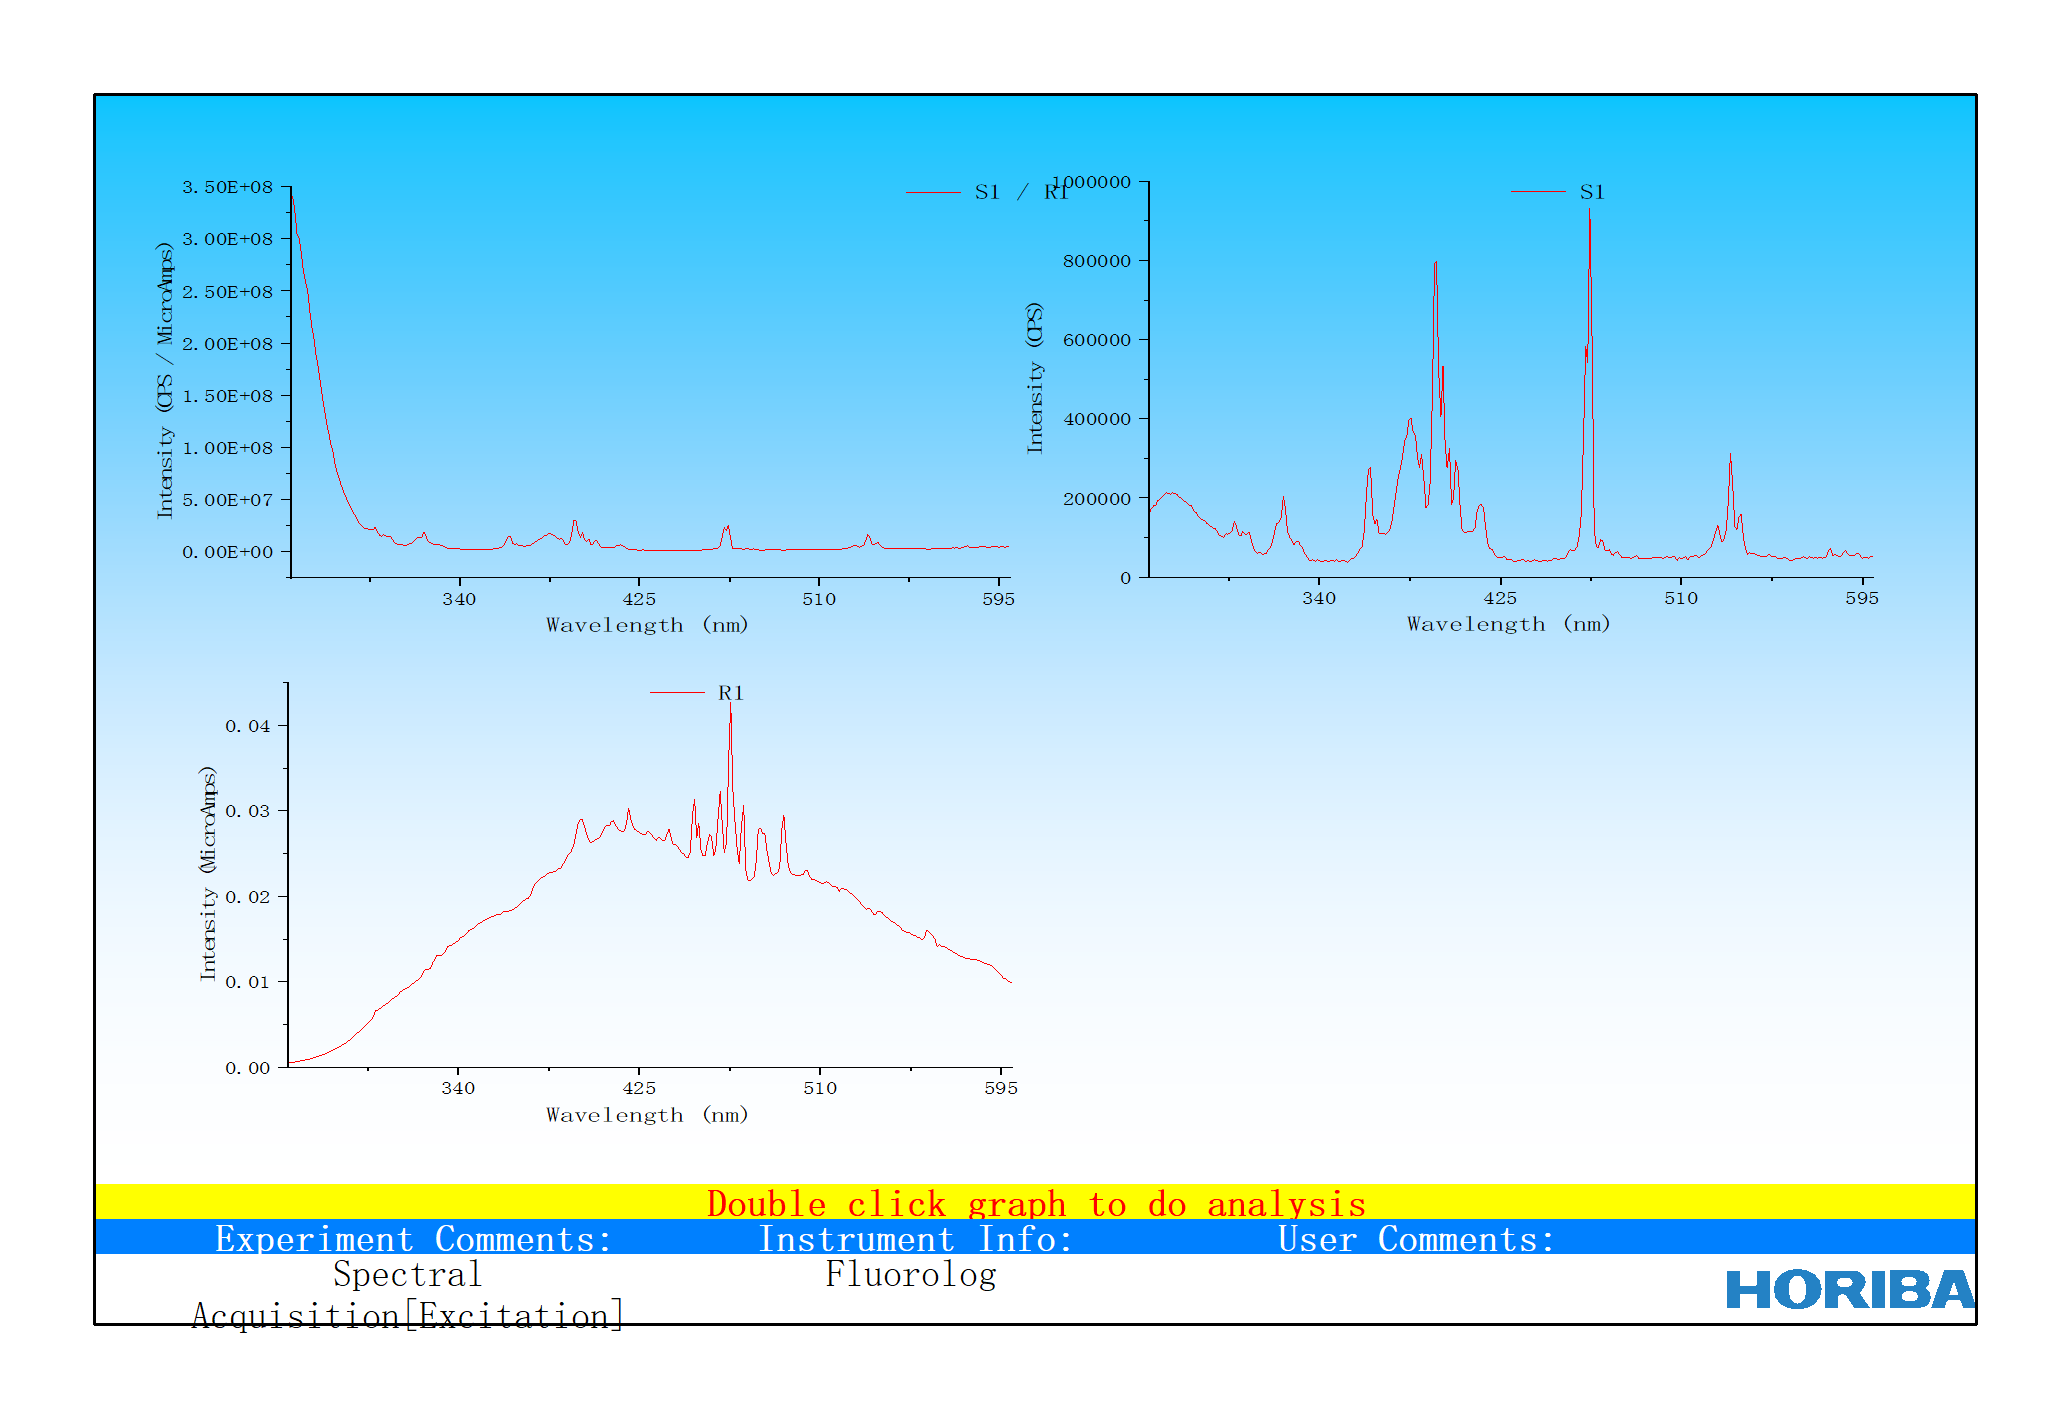
\includegraphics[width = 0.75\linewidth]{RE_Emission_Spectroscopy_611_260-600.png}
		
		需要注意的是,这里得到了三组数据,右上表示单位激发光强下的发射光谱的强度,左下代表在 $611nm$ 处的发射光谱的绝对强度,左上代表激发光的光强随波长的变化。这是因为,在改变激发光波长时,实际上激发光的光强也在改变,激发光的光强必然会影响发射光谱的相对强度,因此讲两者相除,得到单位激发光强下发射光谱的强度,就可以代表该稀土样本的激发光谱。
		
		根据上图,可以发现激发光谱大致随激光波长的增大而减小,这较好理解,波长较小时,光子能量较大,激发光谱的强度较大。此后,还将测量在合适的激发光下,稀土材料在可见光波段的发射光谱。激发光的波长将综合考虑,首先虽然波长较小时激发光谱的强度较大,而由于波长较小时激发光的光强较小,导致发射光谱的强度较小。以此作为参考,选择一个波长较小、发射光谱强度较大的波长,因此 $260nm$ 的激发光波长将是一个合适的选择,重复前面的实验步骤,可以得到发射光谱为:
		
		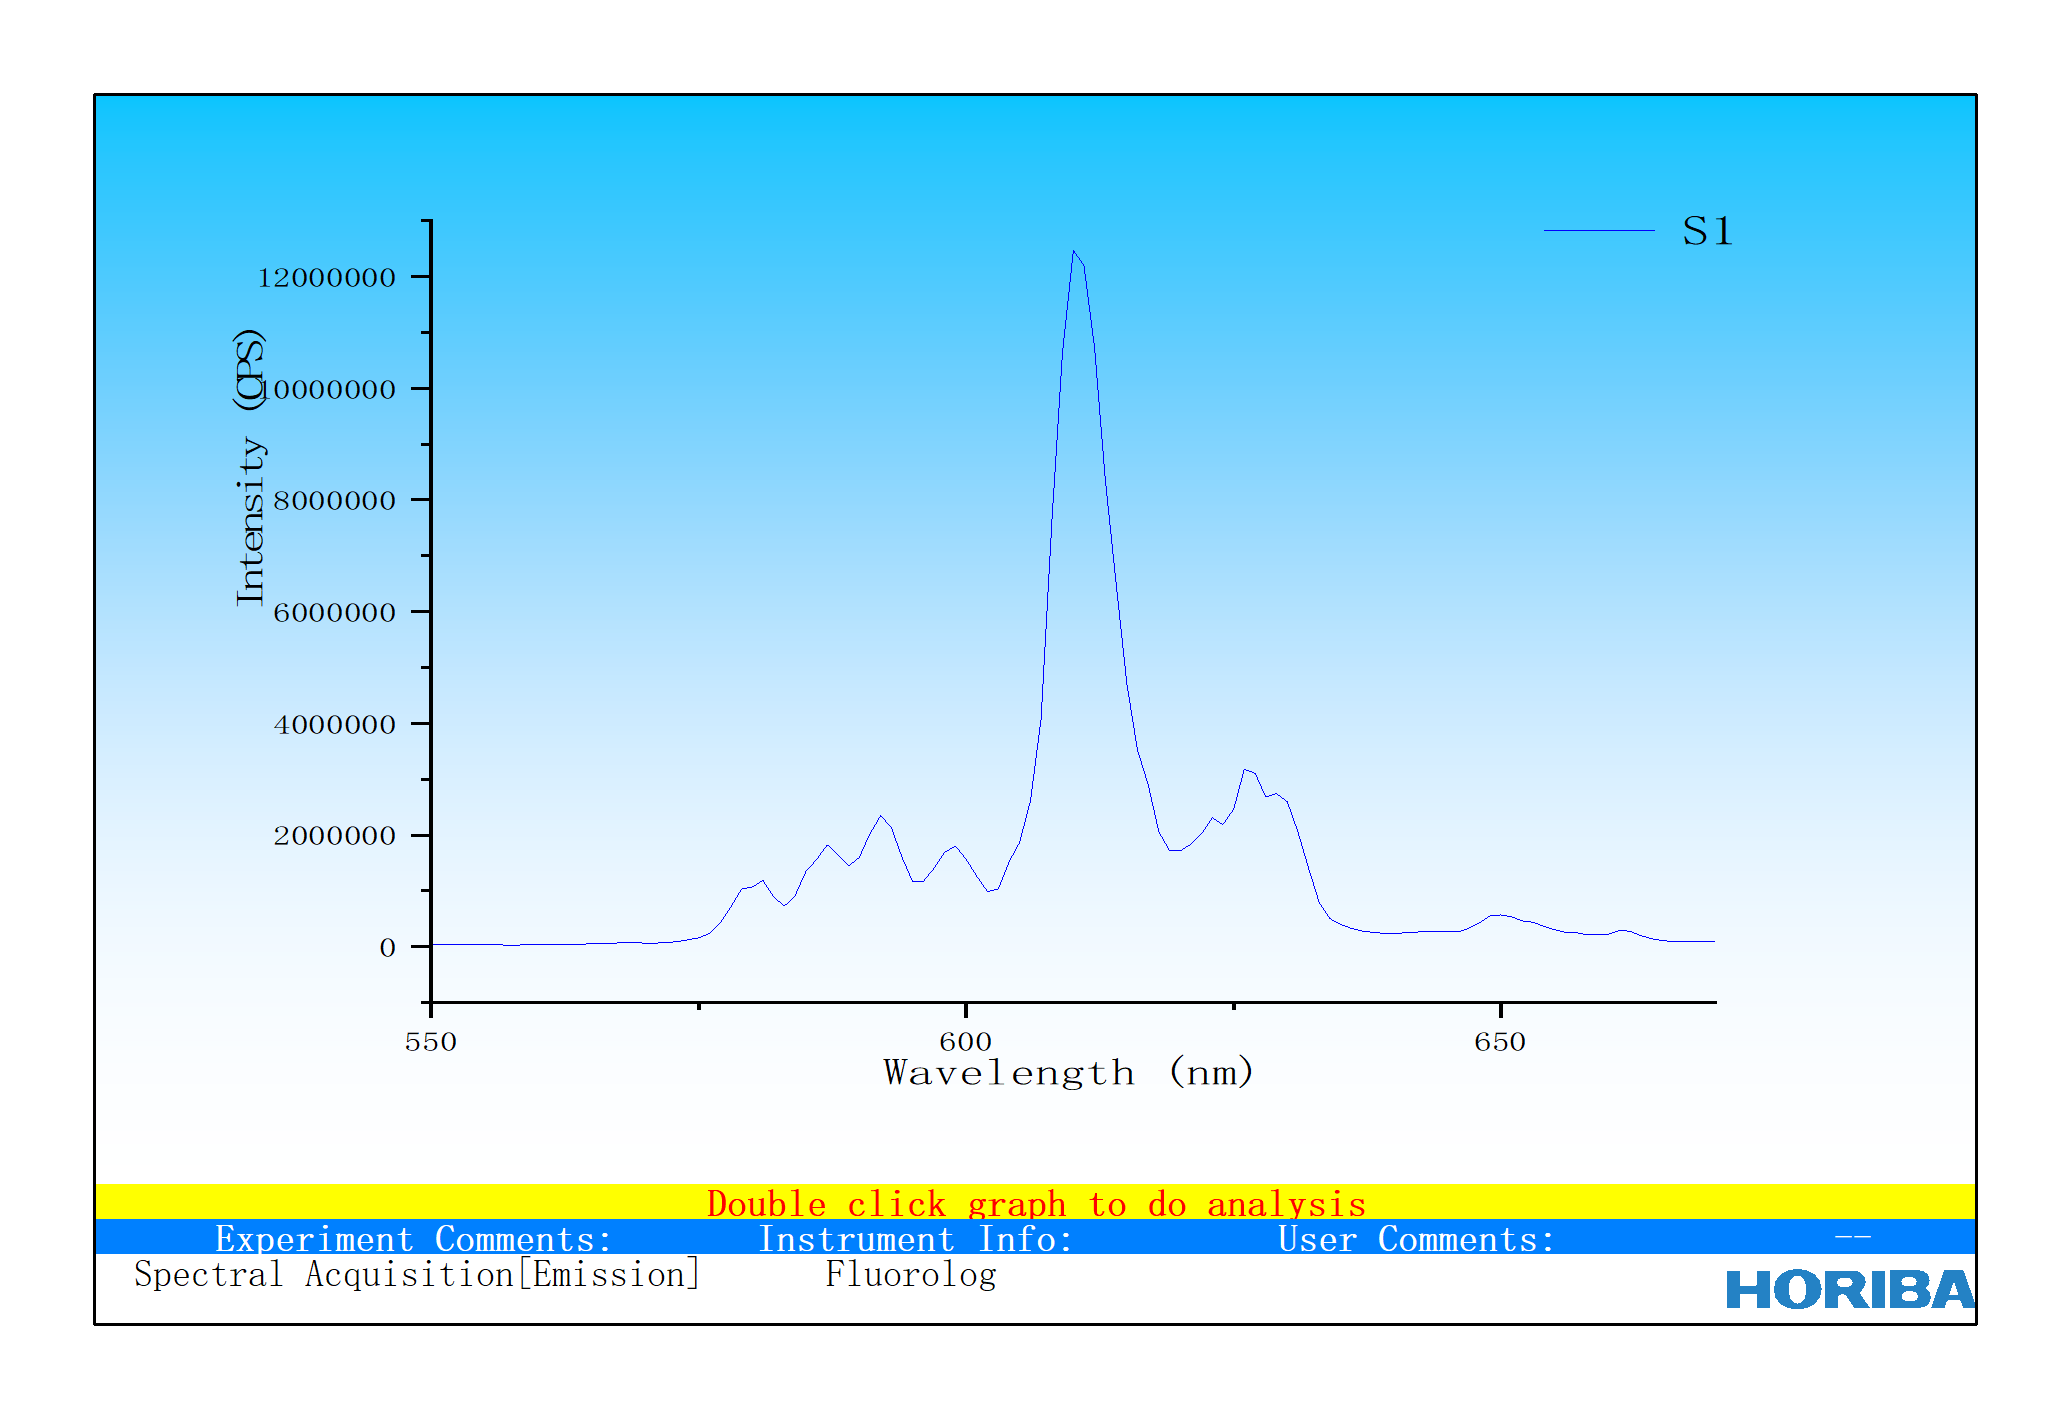
\includegraphics[width = 0.75\linewidth]{RE_Emission_Spectroscopy_550-670_260.png}
		
		可以发现 $600nm$ 与 $650nm$ 波长附近的几个峰值确实为该稀土材料发射光谱的峰值,并不是噪声影响。并且对比激发光波长为 $350nm$ 与 $271nm$ 的两个发射光谱,可以发现波长为 $271nm$ 的发射光谱强度远高于波长为 $350nm$ 的发射光谱强度。至此,我们已经得到了该稀土材料的激发光谱与发射光谱。
		
		\subsection{有机材料的发射光谱}
		考虑波长为 $350nm$ 的激发光,并且入口狭缝为 $5nm$ ,测量其在可见光范围内的发射光谱。注意到实验中仍然使用了长波截至滤光片,只有波长大于 $350nm$ 的光可以通过,因此发射光谱测量范围设置为为 $400-700nm$ ,步长为 $1nm$ 。由此可以得到如下的发射光谱:
		
		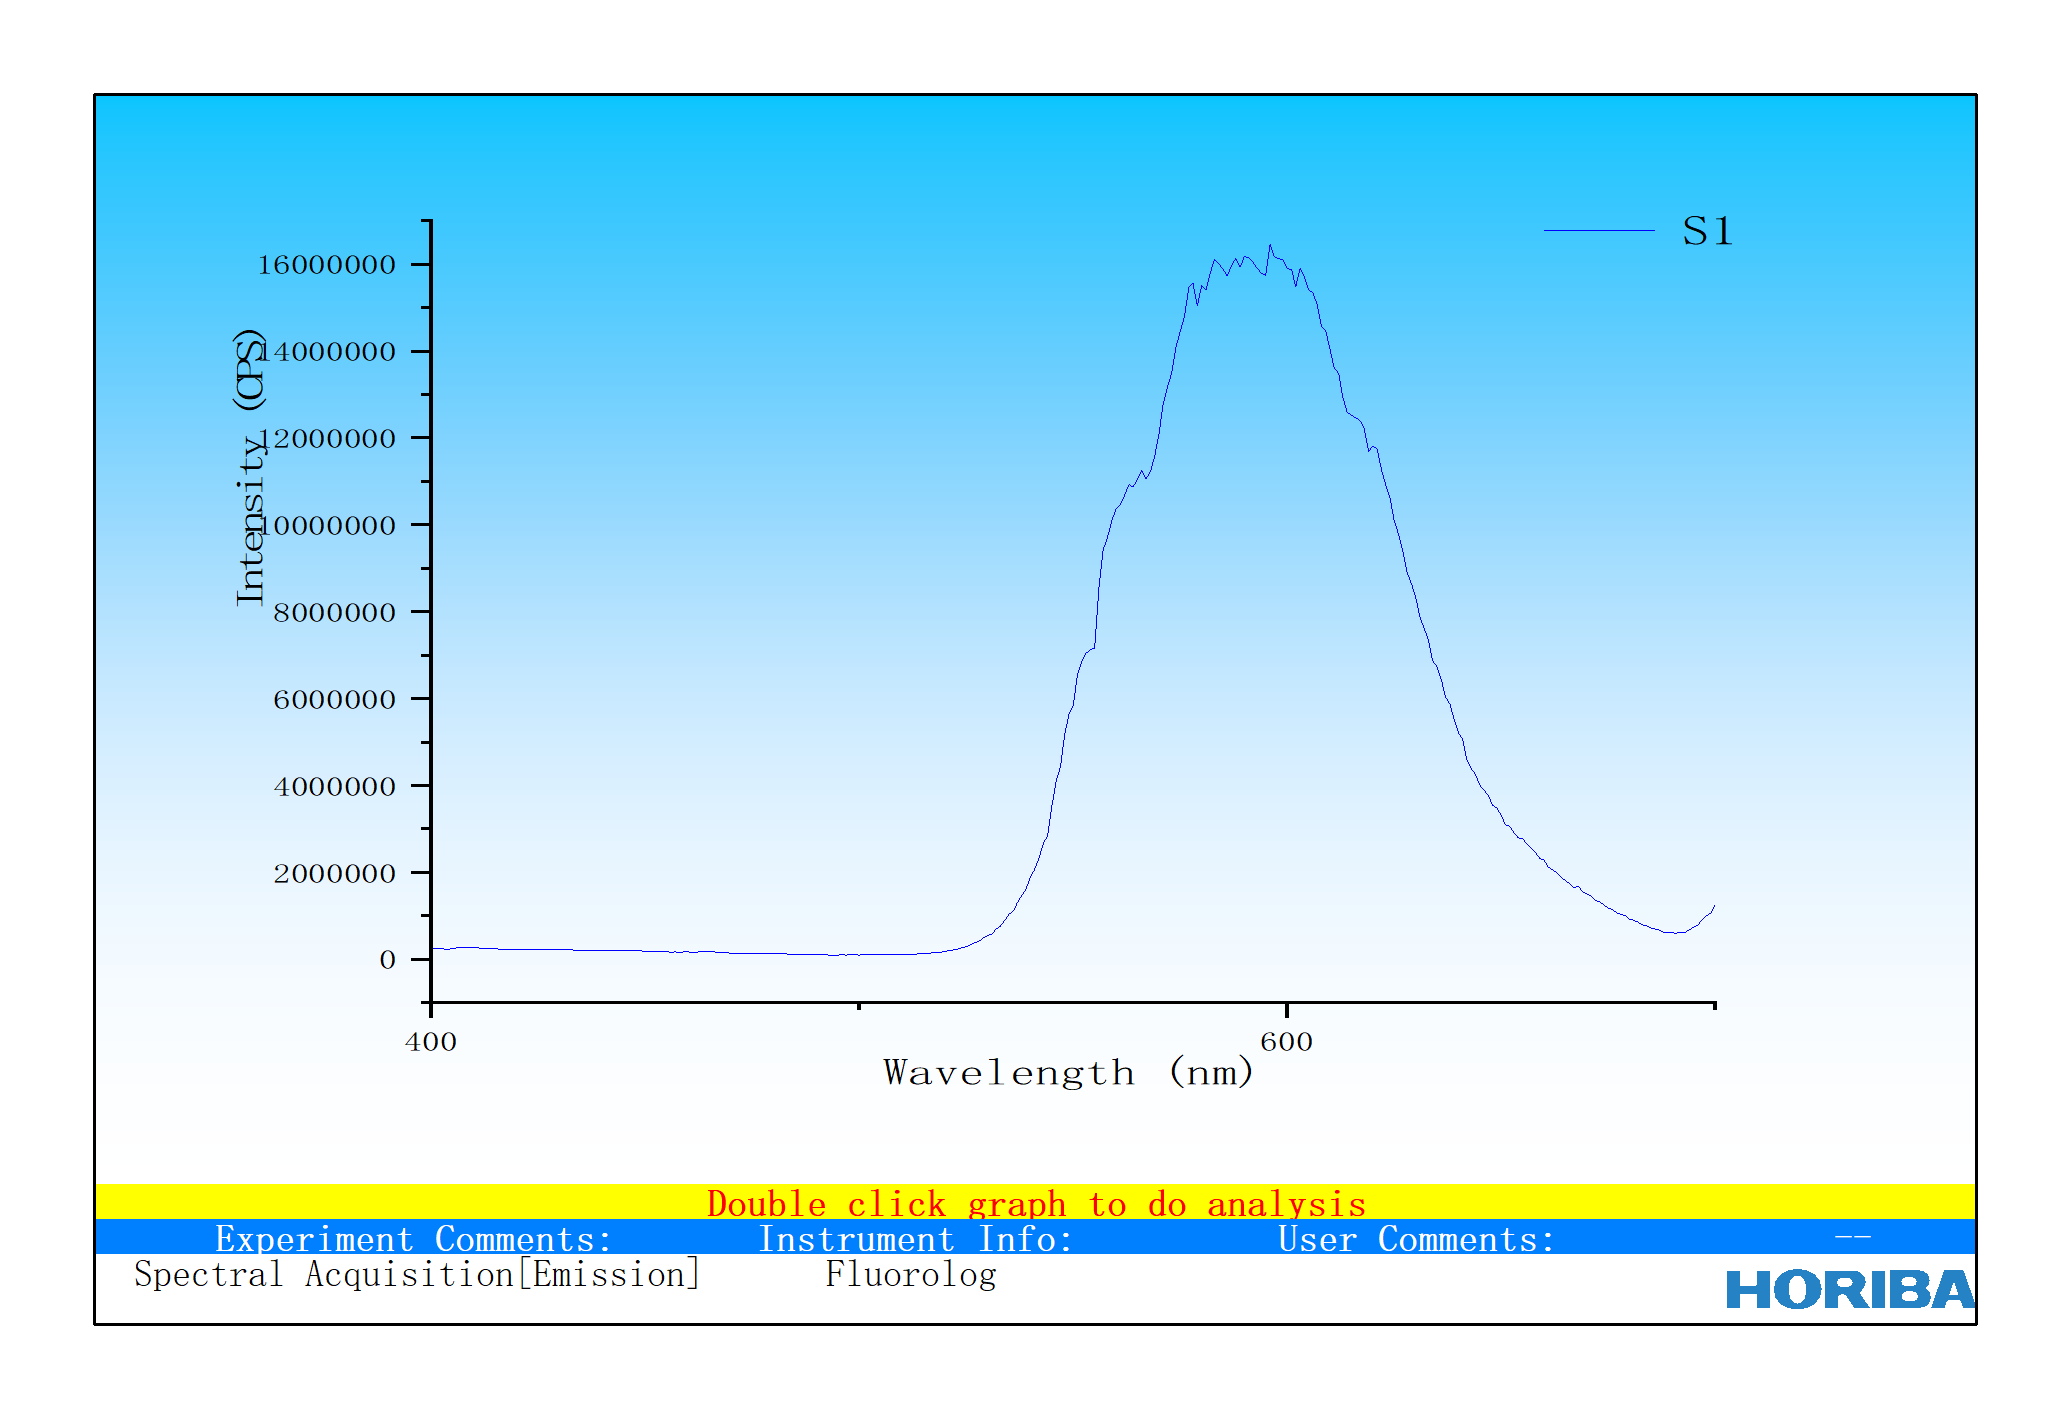
\includegraphics[width = 0.75\linewidth]{OR_Emission_Spectroscopy_400-700_350.png}
		
		定位到其荧光波长极大值位于$600nm$左右。为了更精细定位波长极大值,我们取发射光谱测量范围设置为为 $500-690nm$,测试得到如下的发射光谱:
		
		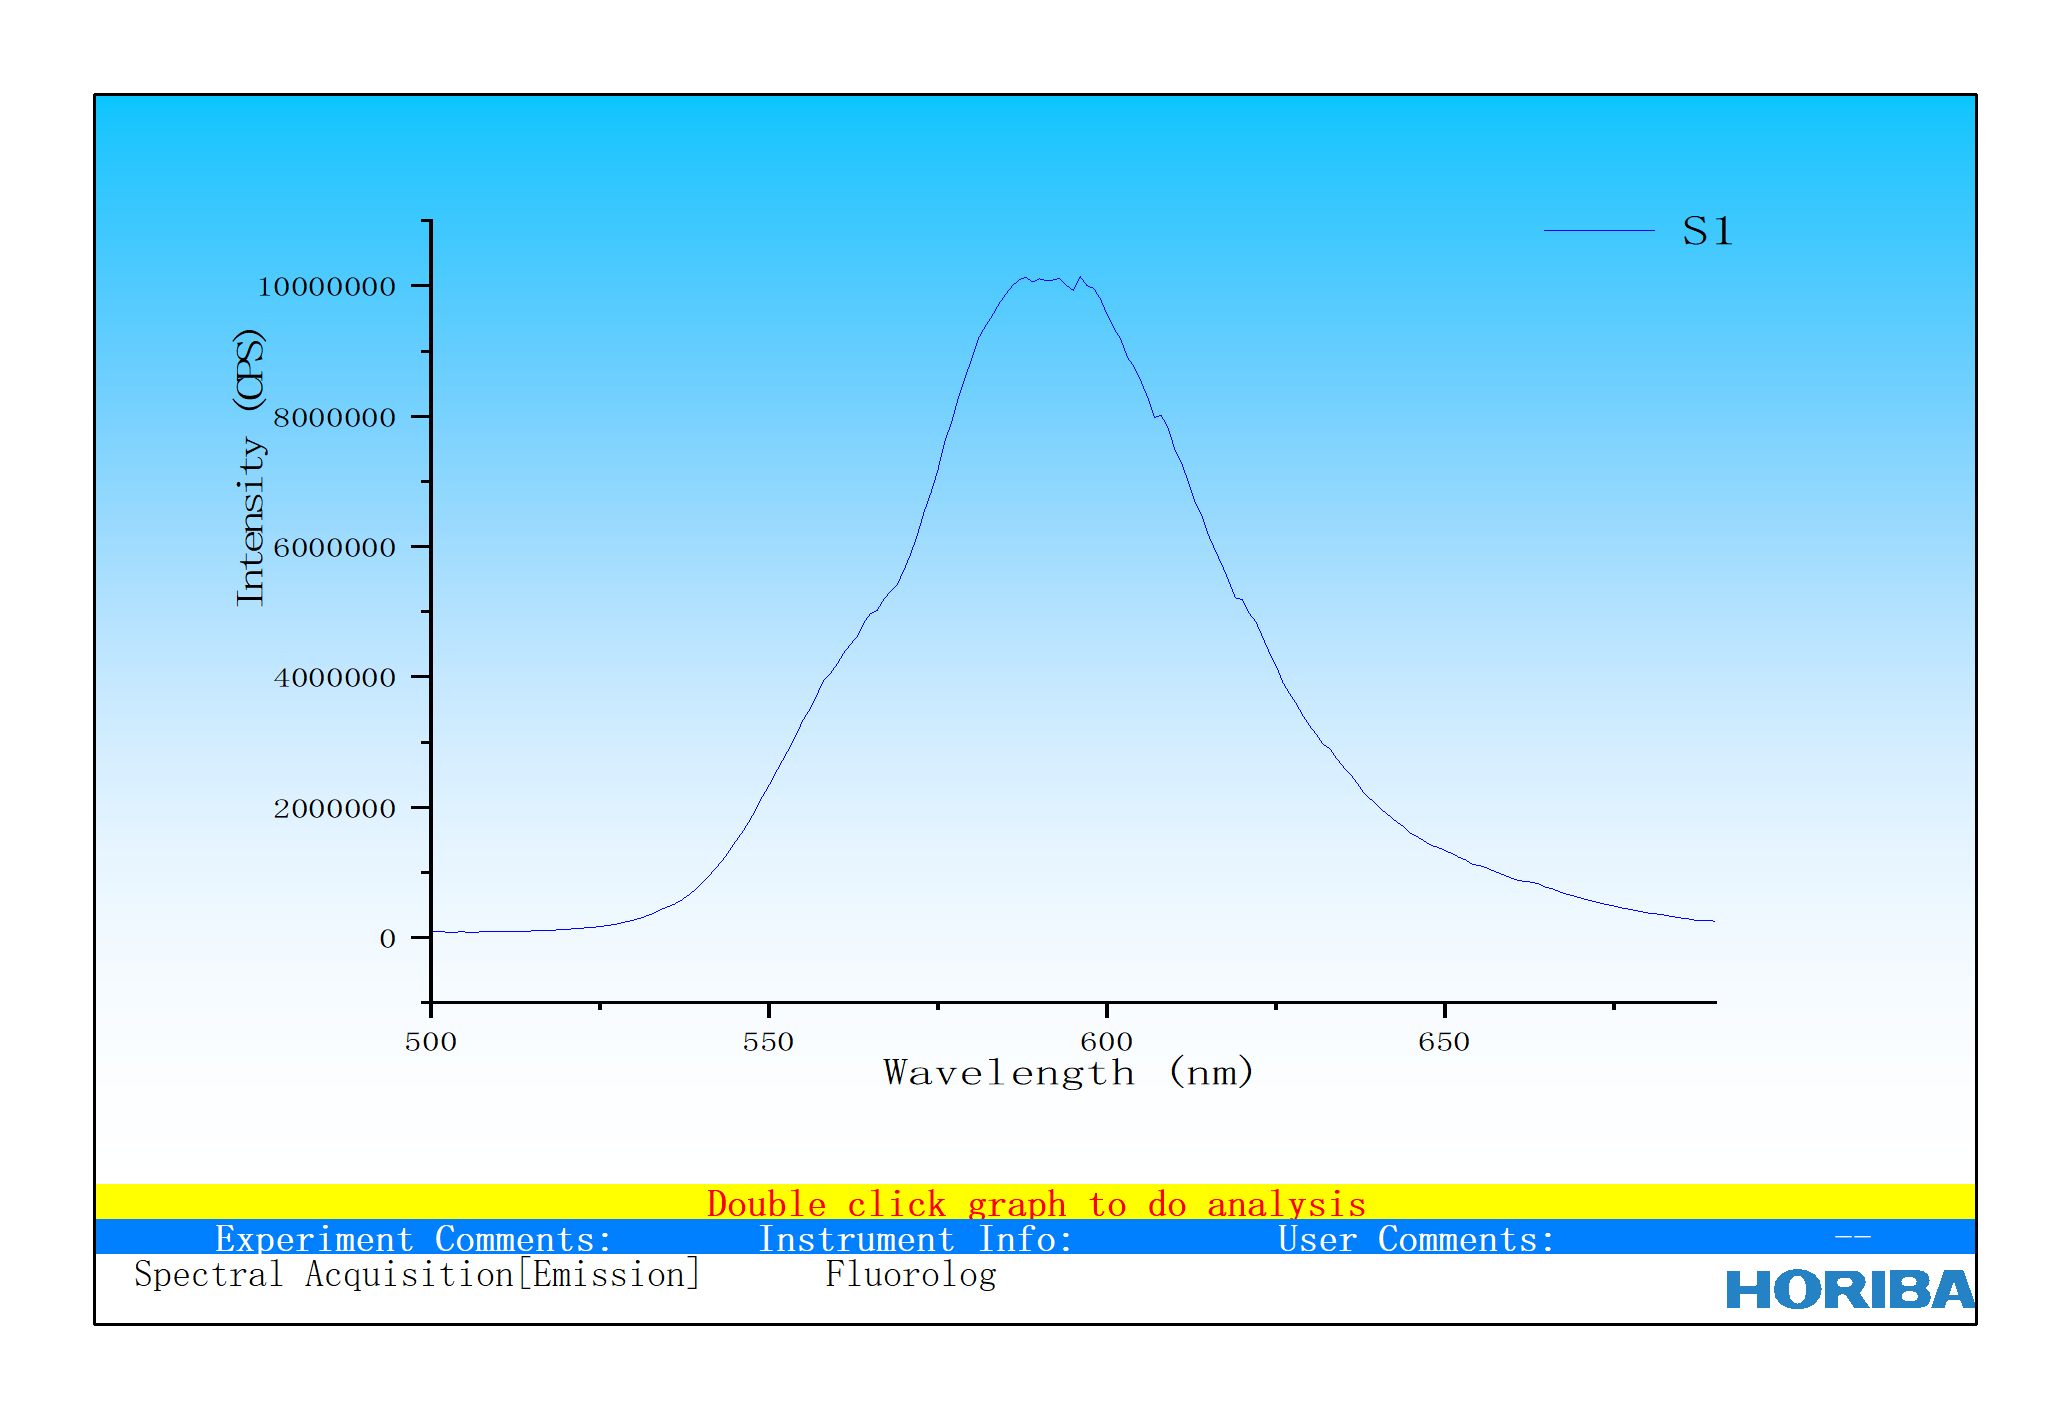
\includegraphics[width = 0.75\linewidth]{OR_Emission_Spectroscopy_500-690_350.png}
		
		可以发现其在 $590nm$ 处存在明显峰值,其他地方并未出现明显峰值。此后,在波长 $590nm$ 处测量其激发光谱,设置激发波长为 $260-600nm$ ,步长为 $1nm$ ,可以得到:
		
		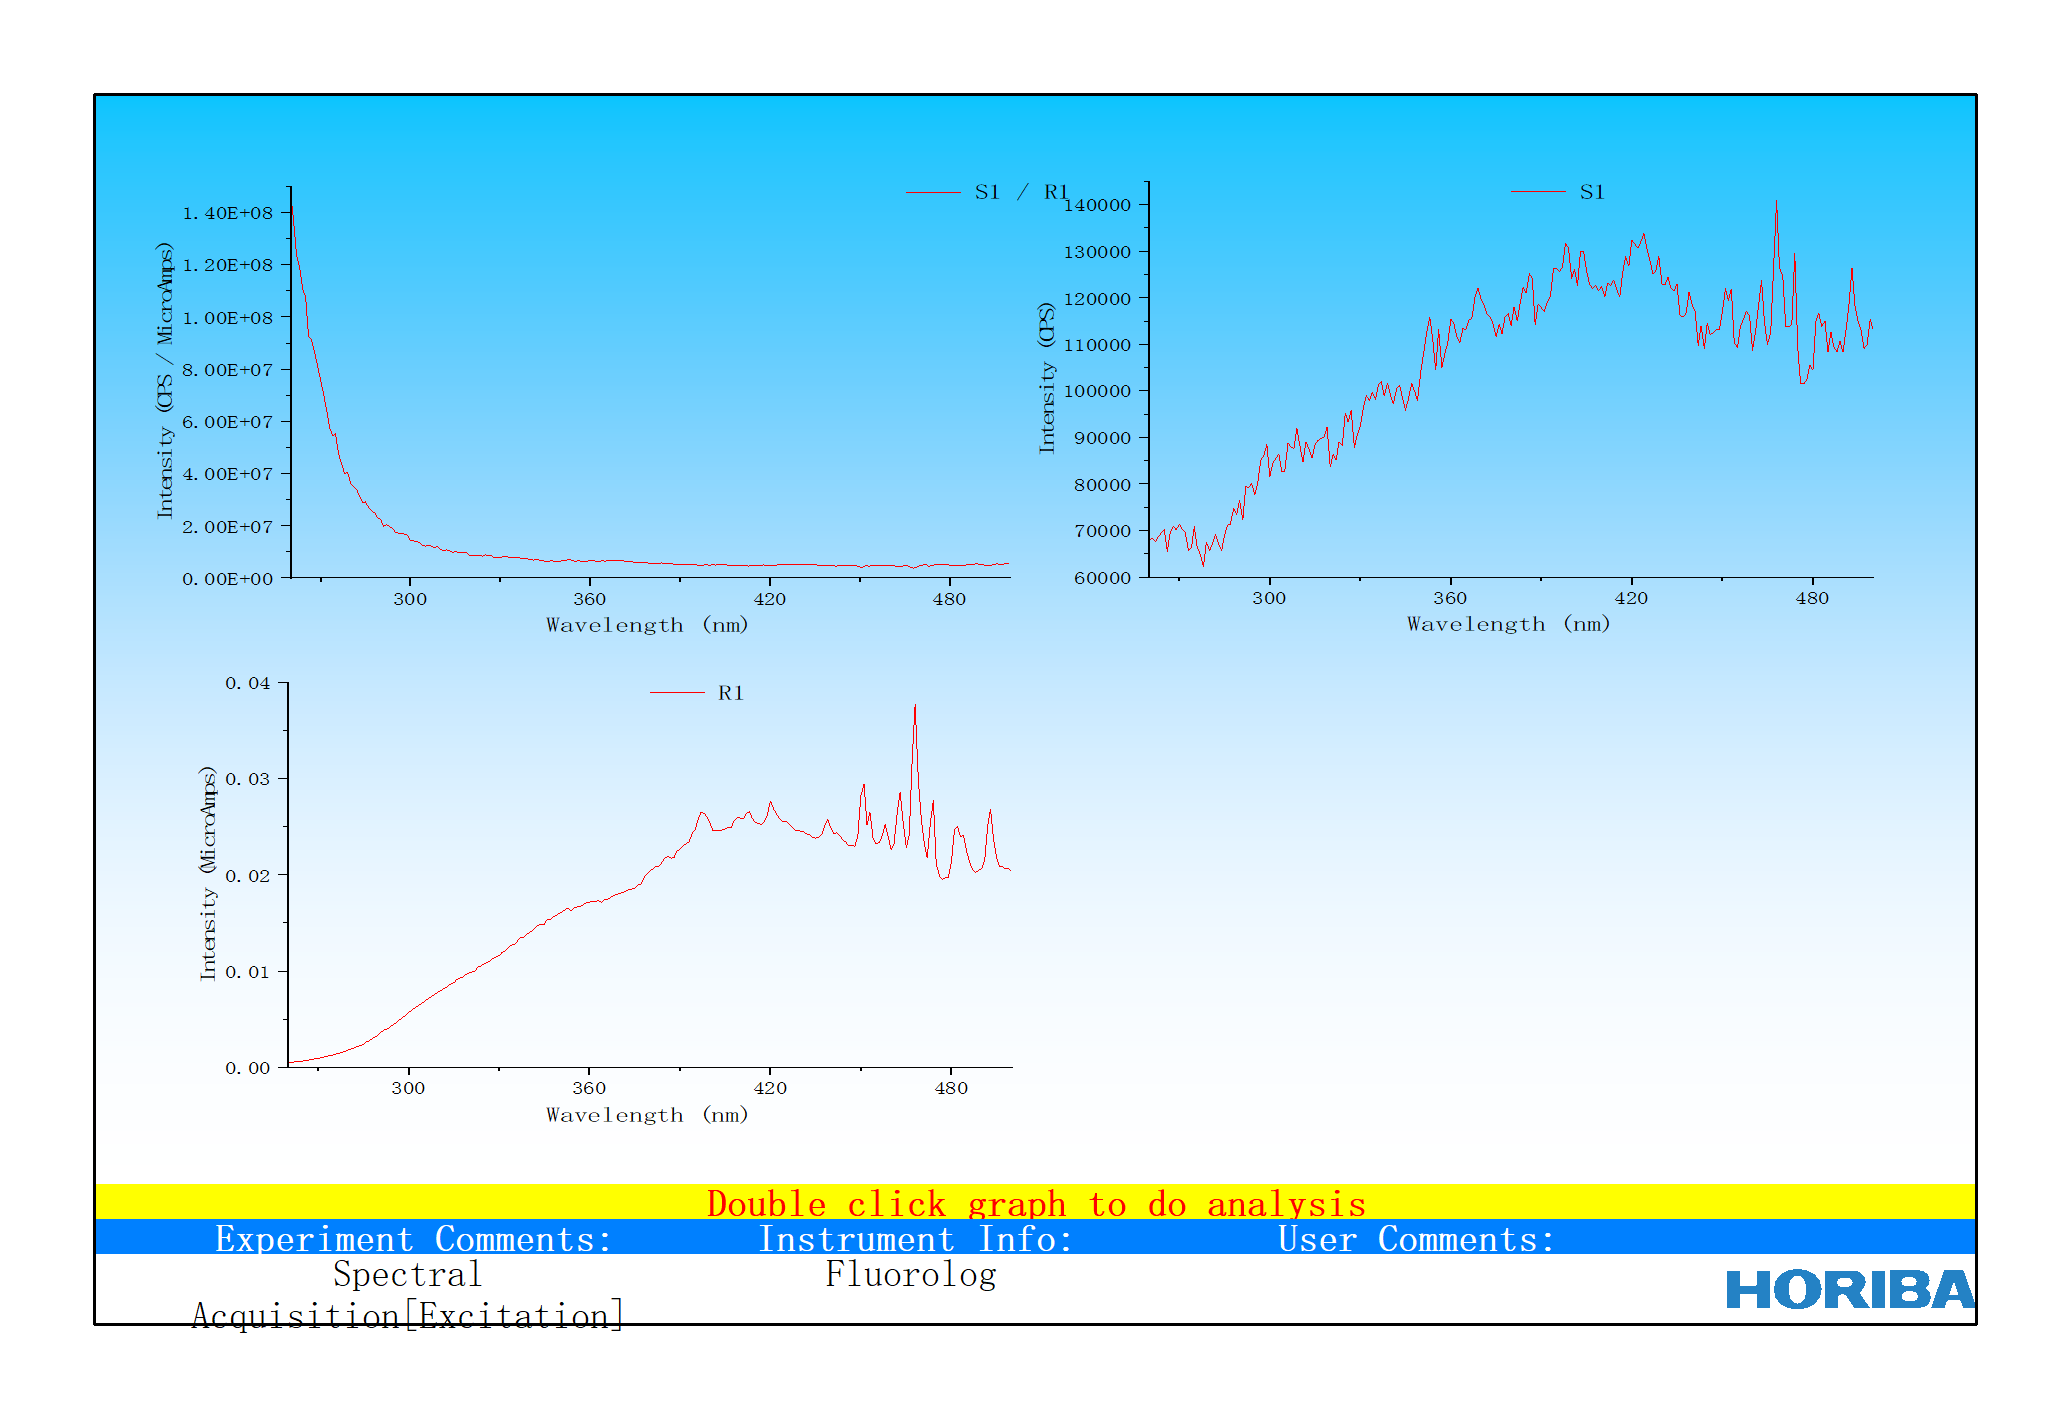
\includegraphics[width = 0.75\linewidth]{OR_Emission_Spectroscopy_590_260-600.png}
		
		可以发现仍是在波长较小的情况下,激发光谱的强度较高。观察图10.2与10.3可以发现,实际上两者的趋势比较相似,并考虑到初次测量有机溶剂的发射光谱时并未发现其他的疑似峰值,此处不再更换其他波长继续测量其发射光谱,不过原则上可以选择一个更加合适的波长进行测量。
		
		\subsection{图像对比分析}
		对比两组材料的图像,我们注意到,稀土材料相对于有机材料,具有明显的单原子特征,即能谱较为锐利,且存在多个峰,能量取值高度量子化;而有机材料的荧光光谱峰则较为弥散,取值较为连续,具有明显的官能团特征(多个例子强耦合在一起,使能级分布连续)。此外,稀土材料因为其原子特征明显,其吸收光谱也具有高度的选择性,选取适当的发射光谱得到的发射强度会显著变大,而有机材料因为其能级分布连续,选择性大大降低,对任何波长的入射光具有相似的荧光发射强度。
		
		有鉴于此,我们提出几种定性可行的材料鉴别方法:
		\begin{enumerate}
			\item	利用主峰的半峰宽来鉴别材料种类
			\item	利用次峰的多少来鉴别材料
			\item	利用荧光强度比值来鉴别材料
		\end{enumerate}
		以上的鉴别方法均在本次实验中有明显体现。可以预见,通过对更多种材料光谱的测量分析,我们可以为这三种鉴别方法提出定量指标,帮助我们更好的分析材料。
		
		\section{总结}
		
		本次实验中,我们测量了稀土材料、有机试剂的激发光谱、发射光谱。我们发现稀土材料的光谱线较为锐利,且存在多个峰,对激发光具有较高的选择性,说明稀土材料的内部结构具有典型的原子个体行为特征;有机材料的光谱线较为弥散,且与激发光的强度关联不大,具有典型的原子团特征。我们进一步根据分析结果提出三种定性分析鉴别物质的方法,并说明其在本次实验中体现出的可行性。
		
		\section{思考题}
		\paragraph{1、根据附录中给出的滤色片的光谱特性,谈谈如何在光路中正确使用JB510和ZWB2这两块滤色片。}
		
		JB510滤色片为长波截止滤色片,在测量红外光谱时使用,放置于红外探测器前的发射单色仪前。
		
		ZWB2滤色片为 $360nm$ 短波截止滤色片,本次实验没有用到。如果需要用到的话,可以用于上转换荧光等荧光光子能量大于激发光的光谱的测量。
		
		
		\paragraph{2.现有两块光栅,刻槽密度分别为 1200条/mm和600条/mm ,请问哪块是可见光栅?哪块是红外光栅?为什么?哪块光栅可能分辨率高些?为什么?}
		
		对于透射光栅,光栅方程为:
		$$
		d \sin{\theta}= m \lambda \qquad m=0,\pm 1,\pm 2 \dots
		$$
		其中 $d$ 为光栅常数,这里分别为:
		$$
		d_1=\frac{1}{1200}mm \approx 833nm \qquad d_2=\frac{1}{600}mm \approx 1667nm
		$$
		因此可以得到,对于两块光栅,波长满足:
		$$
		\lambda_1=\frac{d_1}{m} = \frac{833}{m} nm \qquad m=1,2,3 \dots 
		$$
		$$
		\lambda_2=\frac{d_2}{m} = \frac{1667}{m} nm \qquad m=1,2,3 \dots 
		$$
		因此第一块是可见光栅,第二块为红外光栅。
		
		光栅的色分辨本领为:
		$$
		R=mN=m\frac{D}{d}
		$$
		其中,$D$ 为光栅的尺寸,$d$ 为光栅常数。因此实际上,对于相同大小的光栅,显然刻槽密度 $1200条/mm$ 的光栅分辨率较高。
		
		\paragraph{3. 根据实验中所用探测器的特点,你认为如何才能改进本实验的测量灵敏度。}
		
		\begin{enumerate}
			\item	提高进入探测器光线的单色性。
			\item	提高光线的光强。
			\item	选用合适的滤光片。
		\end{enumerate}
		
		
		
		\section*{鸣谢}
		感谢中国科学技术大学第一教学楼 物理实验教学中心提供的器材支持与教师指导
		
		
		感谢同学和助教的无私解答与帮助
		
		
		\begin{thebibliography}{100}%此处数字为最多可添加的参考文献数量
			\bibitem{article1}荧光光谱实验 实验PPT
			
			
			中国科学技术大学物理实验教学中心\quad 著
			
			\bibitem{article2}荧光光谱实验 实验报告
			
			杨晨\quad 著
			
		\end{thebibliography}
		
	\end{multicols}
\end{document}
